\documentclass[tikz,border=3pt]{standalone}
\usepackage[T1]{fontenc}
\usepackage{amsmath}\usepackage{graphicx}
\usepackage{XCharter}
\usepackage[xcharter]{newtxmath}
\usepackage[scaled=.92]{helvet}
\usepackage{pgfplots}
\usetikzlibrary{arrows.meta,positioning,fit,calc,backgrounds,decorations.pathreplacing,patterns}
\usepgfplotslibrary{groupplots,fillbetween}
\pgfplotsset{compat=1.18}
\definecolor{ink}{HTML}{172536}
\definecolor{rgb}{HTML}{3563B8}
\definecolor{event}{HTML}{17857C}
\definecolor{fusion}{HTML}{76529C}
\definecolor{reference}{HTML}{8994A3}
\definecolor{warn}{HTML}{AC5948}
\definecolor{muted}{HTML}{657183}
\definecolor{rule}{HTML}{D9E0E8}
\definecolor{pale}{HTML}{F5F7FA}
\color{ink}
\tikzset{box/.style={rounded corners=2pt,draw=rule,fill=white,align=center,inner sep=4pt,font=\sffamily\fontsize{9}{10.8}\selectfont,minimum height=9mm},rb/.style={box,draw=rgb!50,fill=rgb!5},eb/.style={box,draw=event!50,fill=event!5},fb/.style={box,draw=fusion!55,fill=fusion!5},arrow/.style={-{Latex[length=1.8mm]},line width=.65pt,draw=muted},note/.style={font=\sffamily\fontsize{8.4}{10.2}\selectfont,align=center,text=muted},heading/.style={font=\sffamily\fontsize{10}{12}\selectfont\bfseries,align=left,text=ink}}
\pgfplotsset{paper/.style={width=15.7cm,height=6cm,axis lines*=left,axis line style={rule},tick style={draw=none},tick label style={font=\sffamily\fontsize{8.8}{10.4}\selectfont,text=muted},label style={font=\sffamily\fontsize{9.4}{11}\selectfont,text=ink},title style={font=\sffamily\fontsize{10}{12}\selectfont\bfseries,text=ink},legend style={draw=none,fill=none,font=\sffamily\fontsize{9}{11}\selectfont,cells={anchor=west}},grid=major,grid style={rule!65,line width=.3pt},minor tick num=0,scaled ticks=false,unbounded coords=jump,clip mode=individual}}

\hyphenpenalty=10000\exhyphenpenalty=10000
\tikzset{box/.append style={font=\sffamily\fontsize{8}{10}\selectfont},
note/.append style={font=\sffamily\fontsize{8}{10}\selectfont}}
% Generated by scripts/make_official_results.py; do not edit by hand.
\providecommand{\OfficialPhasePublishedOverallMiD}{35.80}
\providecommand{\OfficialOverallAbsoluteGain}{9.228548419}
\providecommand{\OfficialBandContributionSubtotal}{9.227548419}
\providecommand{\OfficialDisplayRoundingResidual}{0.0010}
\providecommand{\OfficialCrucialSmallContributionShare}{82.4\%}
\providecommand{\OfficialPhaseOverallMiD}{35.8015}
\providecommand{\OfficialGarlOverallMiD}{45.03}
\providecommand{\OfficialOverallRelativeGain}{20.49\%}
\providecommand{\OfficialPhaseCrucialMiD}{43.5190}
\providecommand{\OfficialGarlCrucialMiD}{53.13}
\providecommand{\OfficialCrucialRelativeGain}{18.09\%}
\providecommand{\OfficialPhaseSmallMiD}{28.2568}
\providecommand{\OfficialGarlSmallMiD}{37.58}
\providecommand{\OfficialSmallRelativeGain}{24.81\%}
\providecommand{\OfficialPhaseLargeMiD}{25.7179}
\providecommand{\OfficialGarlLargeMiD}{40.61}
\providecommand{\OfficialLargeRelativeGain}{36.67\%}
\providecommand{\OfficialPhaseNegativeMiD}{29.9314}
\providecommand{\OfficialGarlNegativeMiD}{31.29}
\providecommand{\OfficialNegativeRelativeGain}{4.34\%}
\providecommand{\OfficialSampleCount}{6,762}
\providecommand{\OfficialPhaseFailureRate}{0.0\%}
\providecommand{\OfficialGarlFailureRate}{0.0\%}
\providecommand{\OfficialPhaseSubmissionID}{1016512}
\providecommand{\OfficialGarlSubmissionID}{817519}

\begin{document}

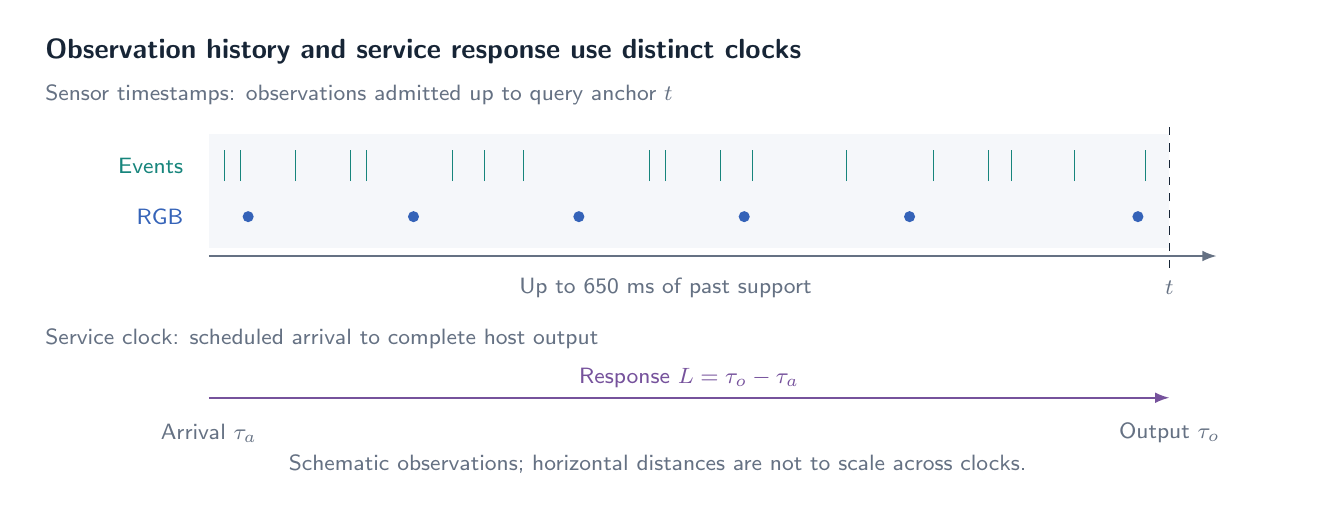
\begin{tikzpicture}[x=1cm,y=1cm]
\path[use as bounding box] (0,-.2) rectangle (16.2,5.5);
\node[heading,anchor=west] at (.1,5.2) {Observation history and service response use distinct clocks};
\node[note,anchor=west] at (.1,4.65) {Sensor timestamps: observations admitted up to query anchor $t$};
\fill[pale] (2.3,2.7) rectangle (14.5,4.15);
\node[note,text=event,anchor=east] at (2.1,3.75) {Events};
\node[note,text=rgb,anchor=east] at (2.1,3.1) {RGB};
\foreach \x in {2.5,2.7,3.4,4.1,4.3,5.4,5.8,6.3,7.9,8.1,8.8,9.2,10.4,11.5,12.2,12.5,13.3,14.2}{\draw[event] (\x,3.55)--(\x,3.95);}
\foreach \x in {2.8,4.9,7,9.1,11.2,14.1}{\fill[rgb] (\x,3.1) circle (2pt);}
\draw[arrow] (2.3,2.6)--(15.1,2.6);
\draw[dashed,ink] (14.5,2.45)--(14.5,4.25);
\node[note] at (8.1,2.2) {Up to 650 ms of past support};
\node[note] at (14.5,2.2) {$t$};
\node[note,anchor=west] at (.1,1.55) {Service clock: scheduled arrival to complete host output};
\draw[arrow,fusion] (2.3,.8)--node[above,note,text=fusion]{Response $L=\tau_o-\tau_a$}(14.5,.8);
\node[note] at (2.3,.35) {Arrival $\tau_a$};
\node[note] at (14.5,.35) {Output $\tau_o$};
\node[note] at (8,-.05) {Schematic observations; horizontal distances are not to scale across clocks.};
\end{tikzpicture}
\end{document}
